\documentclass[oneside]{uniaraxatcc} % Para impressão em frente e verso, utilize twoside
\usepackage[alf]{abntex2cite}
\usepackage[brazil]{babel}
\usepackage{graphicx}
\usepackage{mathtext}
\usepackage{listings}
\usepackage{amssymb}
\usepackage{color}
\usepackage{subcaption}
\usepackage[utf8]{inputenc}
\usepackage{multirow}
\usepackage{scalefnt}
\usepackage{wrapfig}
\usepackage{nomencl}
\usepackage{lipsum}
\usepackage{algorithm}
\usepackage{algpseudocode}

\newcommand{\uniaraxa}{\uppercase{UNIARAXÁ}}

\tipotcc{P} % P:Projeto, M: Monografia
% Nome do Curso
\curso{Sistemas de Informação}

%Qual a habilitação do curso? (Bacharel, Tecnólogo ou Licenciado(a))
\habilitacao{Bacharel}

% Autor(a) do trabalho
\autor{GUILHERME AUGUSTO \\ ISABELLE RESENDE \\ VITOR HUGO DE MORAIS \\ VITOR HUGO RESENDE}

% Título do Trabalho
\titulo{Projeto Integrador - BOT}

% Local cidade / estado
\local{Araxá}{Minas Gerais}


% Data dia / mês / ano da defesa
\date{24}{Novembro}{2022}

%Define a linha de pesquisa
% - Cultura, Desenvolvimento Humano e Gestão
% - Ambiente, Saúde e Políticas Públicas.
% - Produção, inovação e sustentabilidade.
\linhadepesquisa{Cultura e Desenvolvimento de Sistemas}

% Orientador [Tratamento]{Nome}{Gênero: M para Masculino e F para Feminino}
\orientador[Prof. Me]{Humberto Gustavo de Melo}{M}

% Membros da banca, podem ser definidos 2 membros de A a B (sendo que o orientador e o co-orientador já  são membros da banca)

% Primeiro membro da banca (Obrigatório)
\avaliadorA[Profa. Me.]{Nome do Membro 1}{F}

% Segundo membro da banca (Opcional)
\avaliadorB[Prof. Me.]{Nome do Membro 2 (Não obrigatório)}{M}

% Dedicatória (Opcional)
\dedicatoria{Dedicatória não obrigatória. }

% Agradecimentos (Opcional)
\agradecimentos{\noindent\chapter*{\uppercase{Agradecimentos}}

Nossos sinceros agradecimentos ao Me. e Coordenador desse Projeto, Humberto Gustavo de Melo, que nos proporcionou uma grande experiência em diversos aspectos e incentivou a todos a buscar mais conhecimento. Fazendo com que cada um dos envolvidos tenha aprendido e tirado bom proveito de questões diferentes ampliando nossa visão sobre o mundo tecnológico, mercado de trabalho e atualidade. \\

Agradecemos aos nossos colegas de turma que nos inspiraram com seus projetos e ajudaram na nossa trajetória em busca de uma plataforma para configurar o BOT. \\
Também agradecemos a todos que colaboraram com o projeto, testando o BOT, seguindo no Instagram, fornecendo feedbacks e dando conselhos para aprimoramento do projeto.}

% Epígrafe (Opcional)
\epigrafe{\input{Partes/Epigrafe.tex}}

% Resumo (Obrigatório)
\resumo{\noindent\chapter*{\uppercase{Resumo}}

Diante da constante evolução tecnológica, foi se criando a necessidade de adaptação muito alta, pois, com novas tecnologias vem novos conhecimentos. E baseado nisso é nítido que existem muitas pessoas leigas no quesito tecnológico, principalmente no acesso a internet. Consequentemente, há muitos usuários que não sabem do perigo que correm ao acessar a Web de forma ingênua e insegura. \\

Pensando na escassez de conhecimento da Era Tecnológica, a atividade proposta neste semestre, foi criar um BOT, cuja característica principal será auxiliar o usuário com ou sem conhecimento sobre Segurança na Internet. O BOT objetivamente será programado para o usuário interagir com ele, assim irá passando informações sobre maneiras de se proteger ao acessar e como lidar em algumas diversas situações cotidianas que se encontra na internet.
 
\vspace{1cm}

\noindent \textbf{Palavras-chaves}:Dicas de segurança, bot, Projeto integrador, Ensino-aprendizagem, conhecimento.}

% Abstract (Obrigatório)
\abstract{\noindent\chapter*{\uppercase{Abstract}}

In the face of constant technological evolution, the need for very high adaptation was created, because with new technologies comes new knowledge. And based on this, it is clear that there are many lay people in terms of technology, especially in terms of internet access. Consequently, there are many users who are unaware of the danger they are in by naively and insecurely accessing the Web.\\

Thinking about the lack of knowledge in the Technological Age, the activity proposed this semester was to create a BOT, whose main characteristic will be to help the user with or without knowledge about Internet Security. The BOT will objectively be programmed for the user to interact with it, so it will pass on information about ways to protect themselves when accessing and how to deal with some different everyday situations that they find on the internet.

\vspace{1cm}

\noindent \textbf{Palavras-chaves}:Security tips, bot, Integrator project, Teaching-learning, knowledge.}

% Siglas e Abreviações (Opcional)
\siglas{\input{Partes/Siglas.tex}}


\begin{document}
\pretextual %Indica início dos elementos pré-textuais
\maketitle %Elementos Pré-textuais
\textual %Indica início dos elementos textuais
%\pagestyle{simple}

\chapter{\uppercase{Introdução}}
\label{introducao}


A constante busca por informação de forma rápida e eficaz cria a necessidade de ferramentas que ofereçam respostas de forma instantânea. A melhor forma de se conseguir esse resultado é com a utilização de BOT's.

Os BOT's são aplicações de software programados para simular ações e repostas humanas de forma padronizada. Sua utilização mais conhecida é como chat de autoatendimento, onde o usuário apresenta uma dúvida e o BOT oferece diversas opções de respostas e ações para suprir a necessidade do usuário. \cite{bots}

O GUIV SECURITY BOT é um BOT educativo voltado para a disseminação de informações a respeito da segurança cibernética, atrevés de diversas interações dentro do software. Seu uso é indicado para todo tipo de usuário que queira saber sobre como melhorar sua segurança na web e quais os principais tipos de riscos virtuais e como evitá-los.\cite{malware}


% Escrever uma introdução explicando sobre o contexto atual de tecnologias envolvendo bots, objetivo geral do trabalho, objetivos específicos
\section{Problema e Justificativa}
\label{justificativa}

 A falta de conhecimento sobre segurança cibernética, traz enormes riscos e grande vulnerabilidade aos usuários, sejam eles pessoas físicas, jurídicas ou órgãos públicos.\cite{navint} \\
 Comprometendo diversos aspectos tais como: roubo de dados, fraudes em pagamentos, diversos tipos de golpes financeiros, vírus digital, entre outros. \cite{virus}


\section{Objetivos}
\label{objetivos}

%Assumindo que existe um problema a ser resolvido, apresente qual o objetivo de seu projeto de pesquisa. O que você pretende (ou pretendeu) exatamente fazer. Aqui, deve aparecer a principal ``contribuição'' de seu projeto. Qual é a principal ``coisa'' que você pretende/pretendeu fazer? Qual sua principal entrega? Não é necessário criar uma subseção para cada tipo. Pode haver uma única seção, chamada de ``objetivos'' cujo texto divida-se naturalmente em objetivo geral e objetivos específicos, deixando claro qual caso está sendo tratado em cada momento. Para diferenciar o objetivo geral dos objetivos específicos, siga as seguintes diretrizes:

\begin{itemize}
		\item \textbf{Objetivo geral}: Desenvolver um BOT de caráter educativo e instrutivo a respeito da segurança dos acessos da internet e seus meios.
		
		\item \textbf{Objetivos específicos}: Para o desenvolvimento dessa aplicação, será necessário: \\ 
		- Pesquisa de trabalhos relacionados ao que estamos prestes a desenvolver; \\
		- Pesquisa sobre plataformas desenvolvidas para criação de um BOT; \\
		- Análise de questões relacionadas a segurança na internet para complementar o trabalho;
		- Elaborar diversas interações com o BOT como perguntas prováveis de serem feitas e respostas automáticas; \\
		- Realização de testes para validar a eficiência do BOT criado; \\
		- Implementação do ChatBOT \cite{chatbot} em um site criado pelo nosso grupo, onde falaremos também sobre o que foi apresentado da matéria do Projeto Integrador no 2º Período.
		
		
\end{itemize}

\chapter{\uppercase{Trabalhos Correlatos}}
\label{referencial}

A pesquisa sobre um trabalho correlato foi sobre o BOT YAGPDB (Yet Another General Purpose Discord Bot), que é um bot de discord que faz um controle da segurança dos servidores.\cite{yagpdb}

\section{Relação com o que se está sendo feito}

O principal objetivo do BOT abordado é a moderação automática, realizando o controle de segurança e privacidade do servidor, podendo proibir links de sites, palavras ofensivas e termos de baixo calão. Com essas funções, o BOT auxilia na gestão do servidor, mantendo o chat seguro e amigável.

A relação com o trabalho que se está sendo feito segue pelo âmbito de que ambos possuem o tema segurança, sendo o trabalho pesquisado, um modo de controle dos conteúdos a serem colocados no discord, e, o que se está sendo feito, um modo de dar dicas e conhecimento sobre segurança cibernética.

 % Descrever o objetivo do trabalho que você pesquisou;
 % qual a relação com seu trabalho; 
 % o que tem diferente entre seu trabalho e o pesquisado.
\section{Foi utilizado algo?}
 
No desenvolvimento do BOT, não foram utilizados nenhum recurso ou programa presentes no trabalho utilizado para pesquisa.

% Você utilizou algo que tem nesse trabalho, se sim ? o que? 
\chapter{\uppercase{Construção do Projeto}}
\label{Construção do Projeto}

\section{Técnologias Utilizadas}

 Inicialmente no projeto, as interações foram desenvolvidas dentro da plataforma Landbot, porém, devido a falta de atenção do grupo em não fazer uma pesquisa sobre a plataforma em questão, após o início do projeto, veio a conhecimento de que a Landbot não possuía um plano gratuito, apenas um período de teste. Outra plataforma considerada foi a IBM, porém esta não disponibiliza um plano gratuito sem o cadastro de um cartão de crédito. \cite{ibm}
 
 Devido a este contratempo, foi necessário fazer uma nova pesquisa de plataformas. Na escolha da plataforma Code7 Boteria, foram levadas em consideração: a disponibilidade de um plano gratuito amplo, possuir opções de coleta de informações disponibilizadas em relatórios e a opção para que o usuário possa dar dicas de falhas e sugestões para melhorias no BOT.

 Após mais pesquisas foi decidido pelo grupo uma outra plataforma, a plataforma escolhida foi a WhatsAuto  \cite{whats}, uma plataforma em formato de aplicativo que se configura para se ter respostas automáticas de uma ampla grade de aplicativos, como mostra na figura abaixo:

\begin{figure}[!htb]
\centering
\captionsetup[subfigure]{labelformat=empty}
\caption{``Aplicativos Suportados''}
\begin{subfigure}{.5\textwidth}
\centering
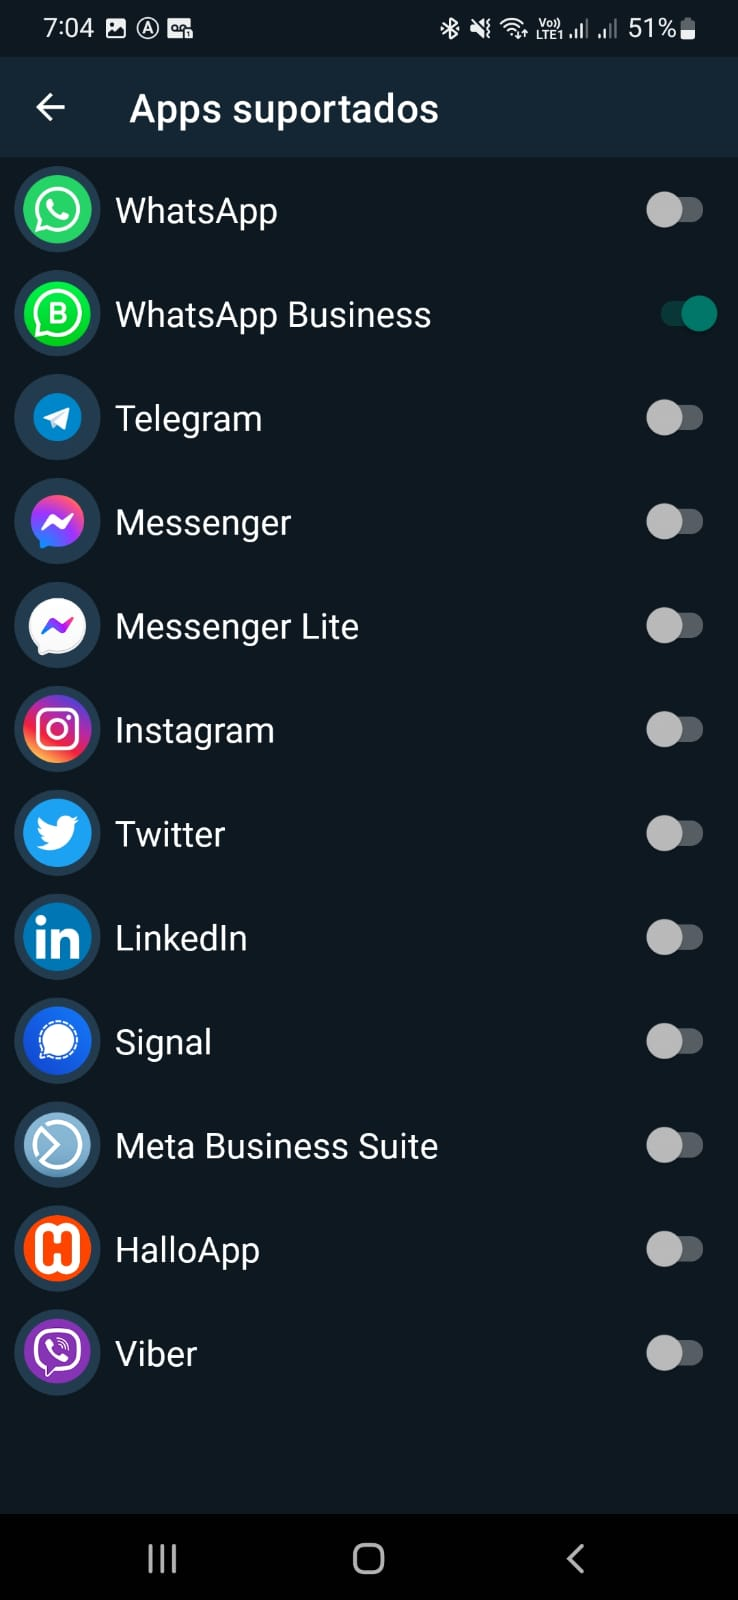
\includegraphics[width=6cm,height=9cm]{Partes/Imagens/Apps Suportados.jpeg}
\caption{Fonte: Criada pelo autor(2022).}
\end{subfigure}%
\end{figure}

Um ponto positivo para a nova plataforma é a facilidade para analisar as estatísticas de respostas, ou seja, o que os usuários mais estão acessando no BOT, dando uma ampla ideia do que melhorar futuramente ou dar mais informações:

\begin{figure}[!htb]
\centering
\captionsetup[subfigure]{labelformat=empty}
\caption{``Estatisticas de respostas''}
\begin{subfigure}{.5\textwidth}
\centering
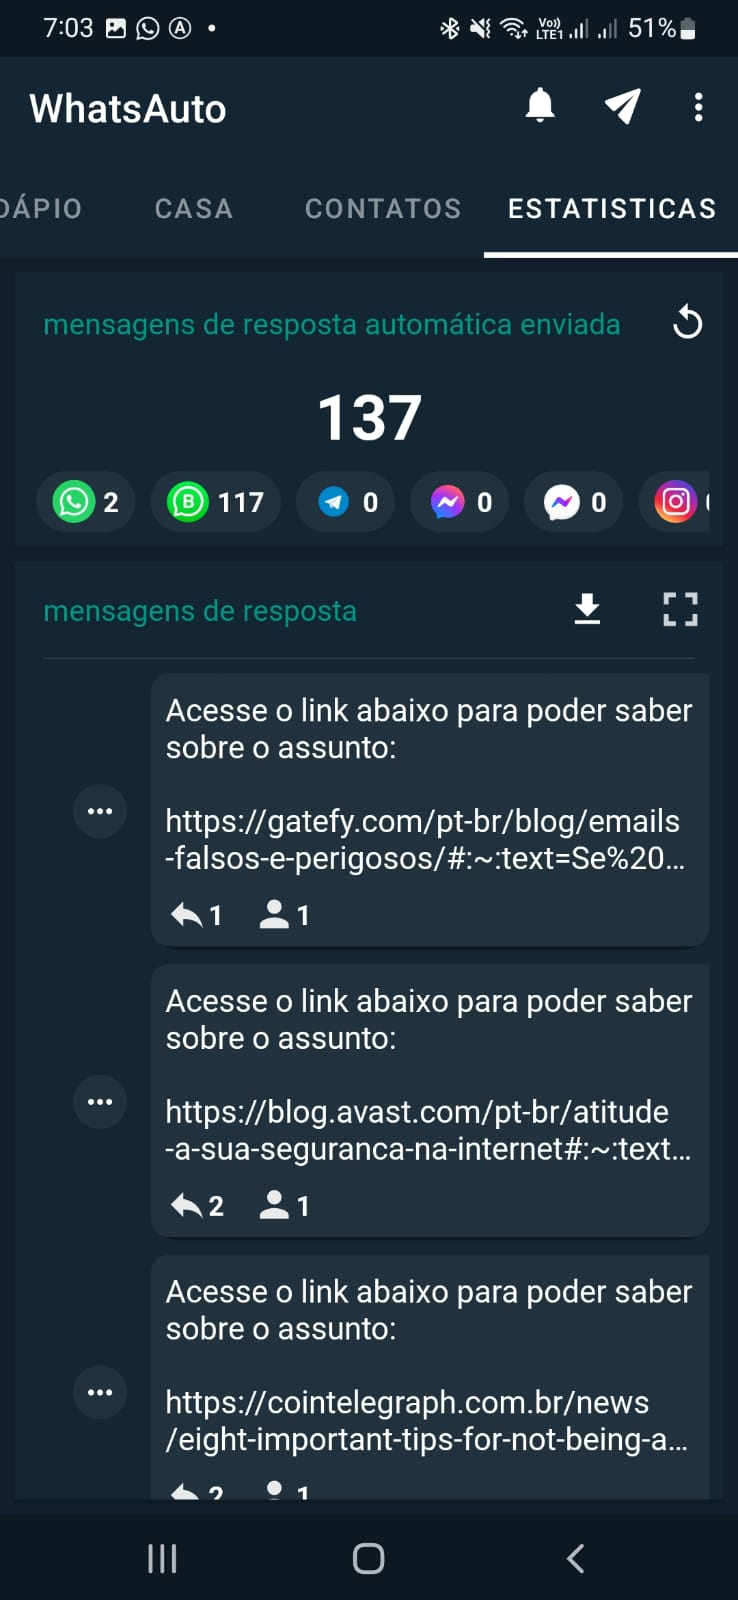
\includegraphics[width=6cm,height=9cm]{Partes/Imagens/Estatisticas.jpeg}
\caption{Fonte: Criada pelo autor(2022).}
\end{subfigure}%
\end{figure}

        \newpage
% Tecnologias utilizadas - Colocar as tecnologias utilizadas e os motivos das escolhas (se tiver custo coloque, se tiver limitação por ser trial, coloque).

% Desenhe um mapa de perguntas e respostas que o bot será capaz de responder.

\section{Protótipo}

A ideia para o nome do BOT veio das iniciais dos integrantes do grupo desenvolvedor, sendo eles: Guilherme, Isabelle, Vitor Hugo de Morais e Vitor Hugo Resende. Assim, foi criado o nome GUIV SECURITY BOT.

\begin{figure}[!htb]
\centering
\captionsetup[subfigure]{labelformat=empty}
\caption{``GUIV''}
\begin{subfigure}{.5\textwidth}
\centering

\includegraphics[width=8cm,height=6cm]{Partes/Imagens/Guiv S.jpeg}
\caption{Fonte: Criada pelo autor(2022).}
\end{subfigure}%
\end{figure}

\begin{itemize}

		\item \textbf{Passo a passo}: 

        O BOT utilizado é um aplicativo de respostas automáticas, que tem vários tipos de modos de respostas como mostra abaixo: \newpage	

\begin{figure}[!htb]
\centering
\captionsetup[subfigure]{labelformat=empty}
\caption{``Opções''}
\begin{subfigure}{.5\textwidth}
\centering
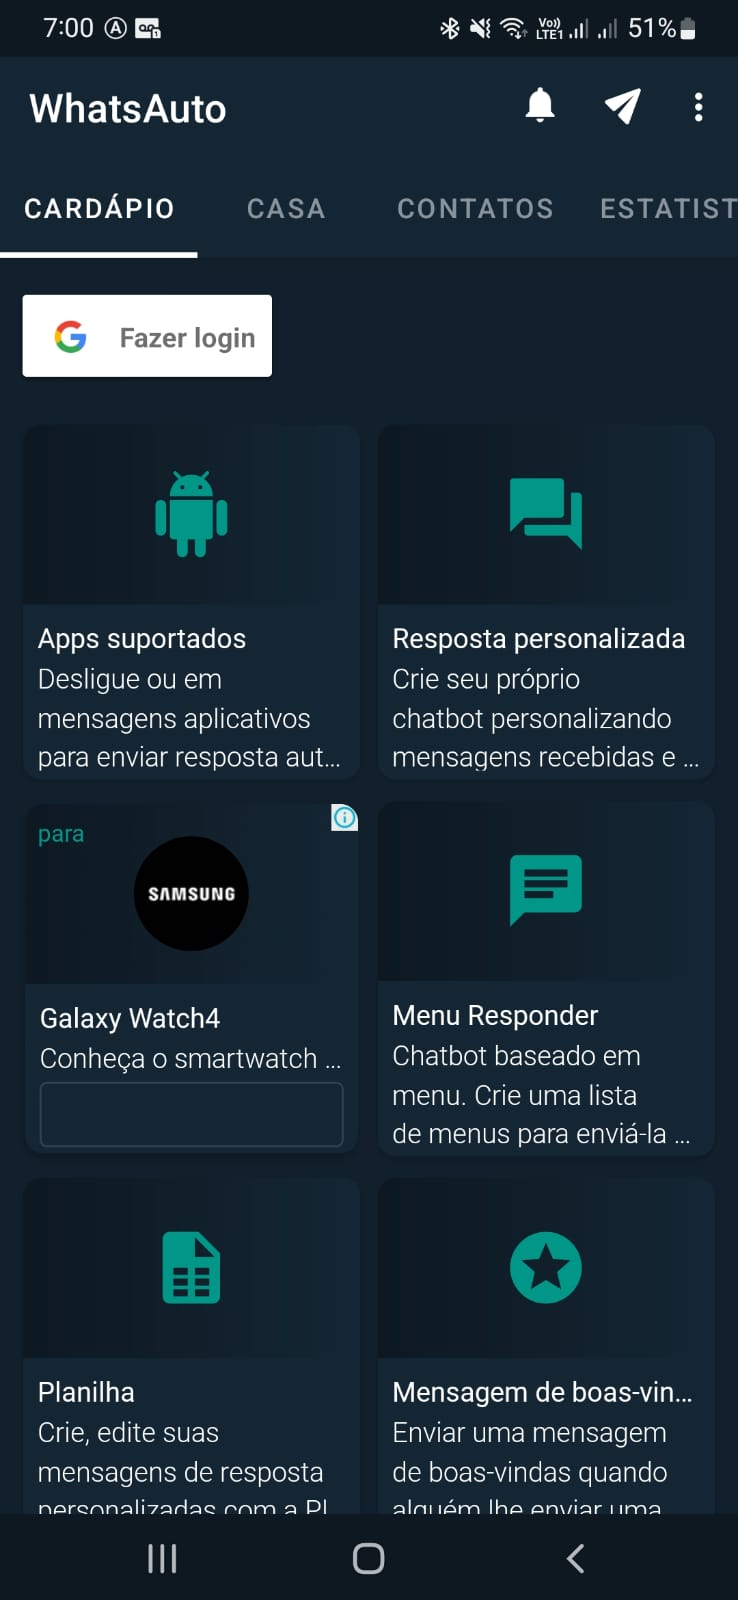
\includegraphics[width=6cm,height=8cm]{Partes/Imagens/Opções.jpeg}
\caption{Fonte: Whatsauto (2022).}
\end{subfigure}%
\end{figure}

        O modo que foi escolhido para fazer o BOT foi o de "Menu Responder", que é um tipo que o BOT te dá opções de respostas, mas além dele, tem opções de respostas que se derivam de mensagens específicas e outras. \\

        Para realizar a criação das opções que o BOT irá te dar para que se possa escolher e ter suas respostas, basta selecionar a opção "Menu Responder", que ele te direcionar a essa tela:  \newpage

\begin{figure}[!htb]
\centering
\captionsetup[subfigure]{labelformat=empty}
\caption{``Menu 1''}
\begin{subfigure}{.5\textwidth}
\centering
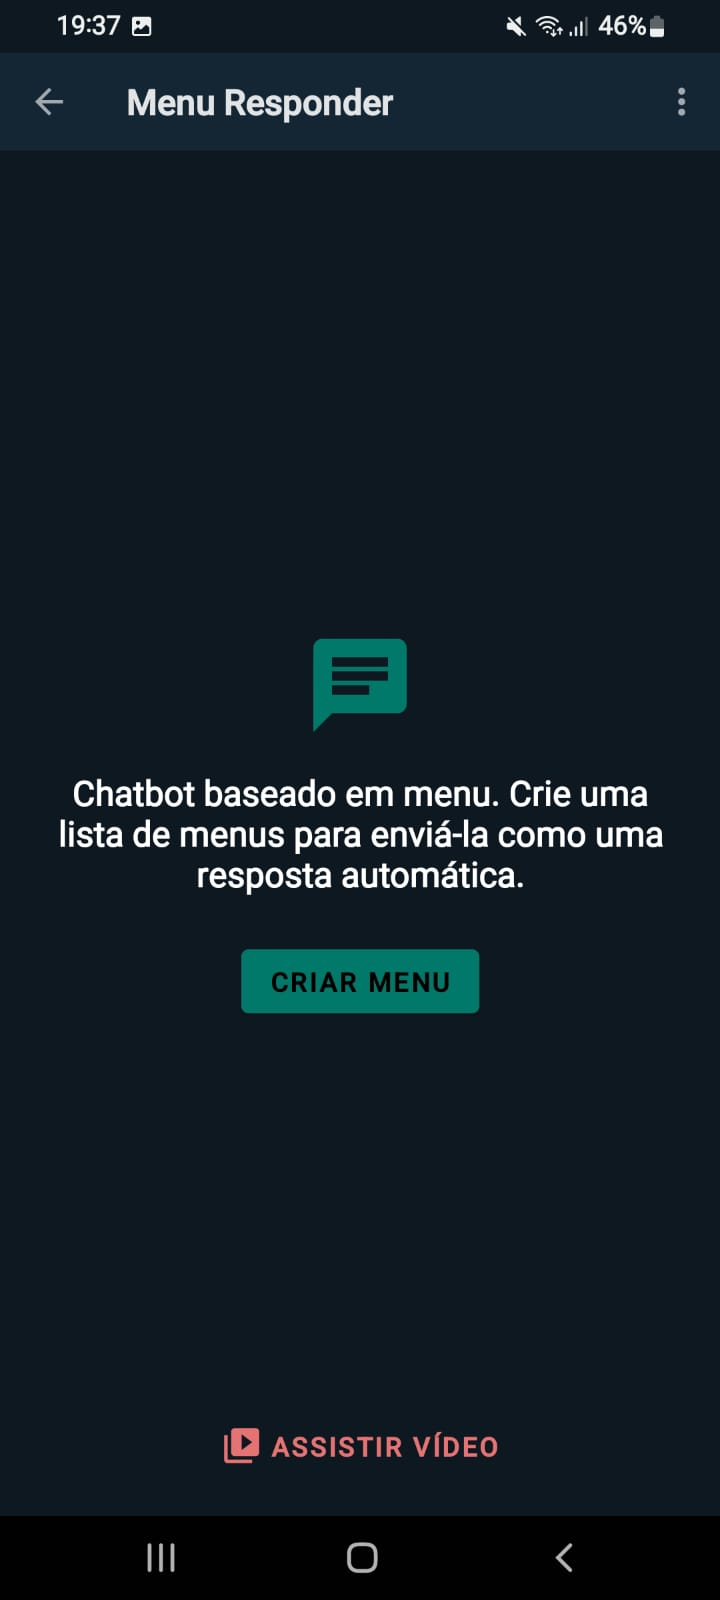
\includegraphics[width=6cm,height=8cm]{Partes/Imagens/Menu 1.jpeg}
\caption{Fonte: Whatsauto (2022).}
\end{subfigure}%
\end{figure}

        Ao abrir essa tela basta clicar em "Criar Menu" que ele te direcionará para a tela de criação:

\begin{figure}[!htb]
\centering
\captionsetup[subfigure]{labelformat=empty}
\caption{``Menu 2''}
\begin{subfigure}{.5\textwidth}
\centering
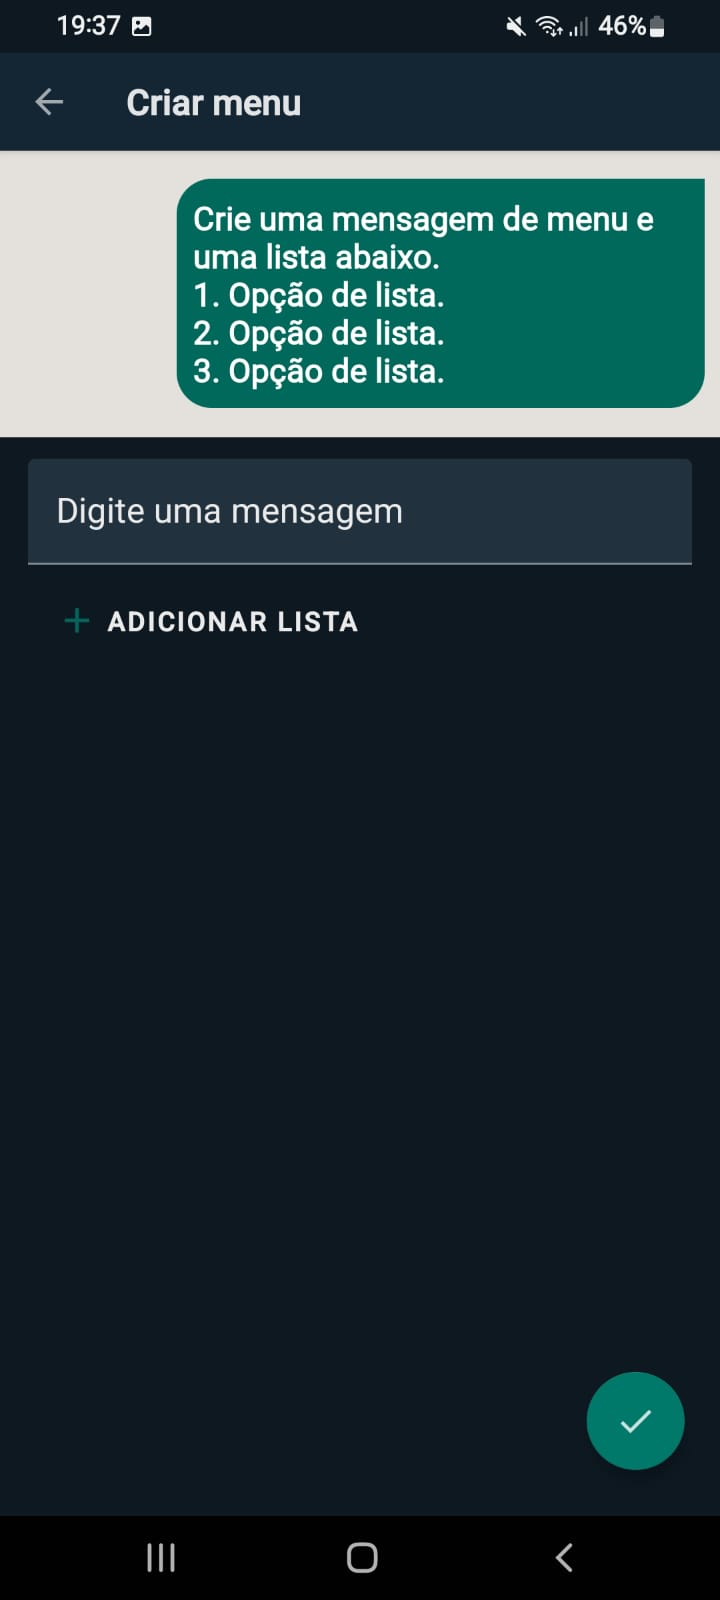
\includegraphics[width=6cm,height=8cm]{Partes/Imagens/Menu 2.jpeg}
\caption{Fonte: Whatsauto (2022).}
\end{subfigure}%
\end{figure}

        Nessa tela você irá colocar um texto inicial e as opções que terá no menu, colocando as informações e clicando na certo verde no canto inferior direito, você irá para a tela de menu criado: \newpage

\begin{figure}[!htb]
\centering
\captionsetup[subfigure]{labelformat=empty}
\caption{``Menu 3''}
\begin{subfigure}{.5\textwidth}
\centering
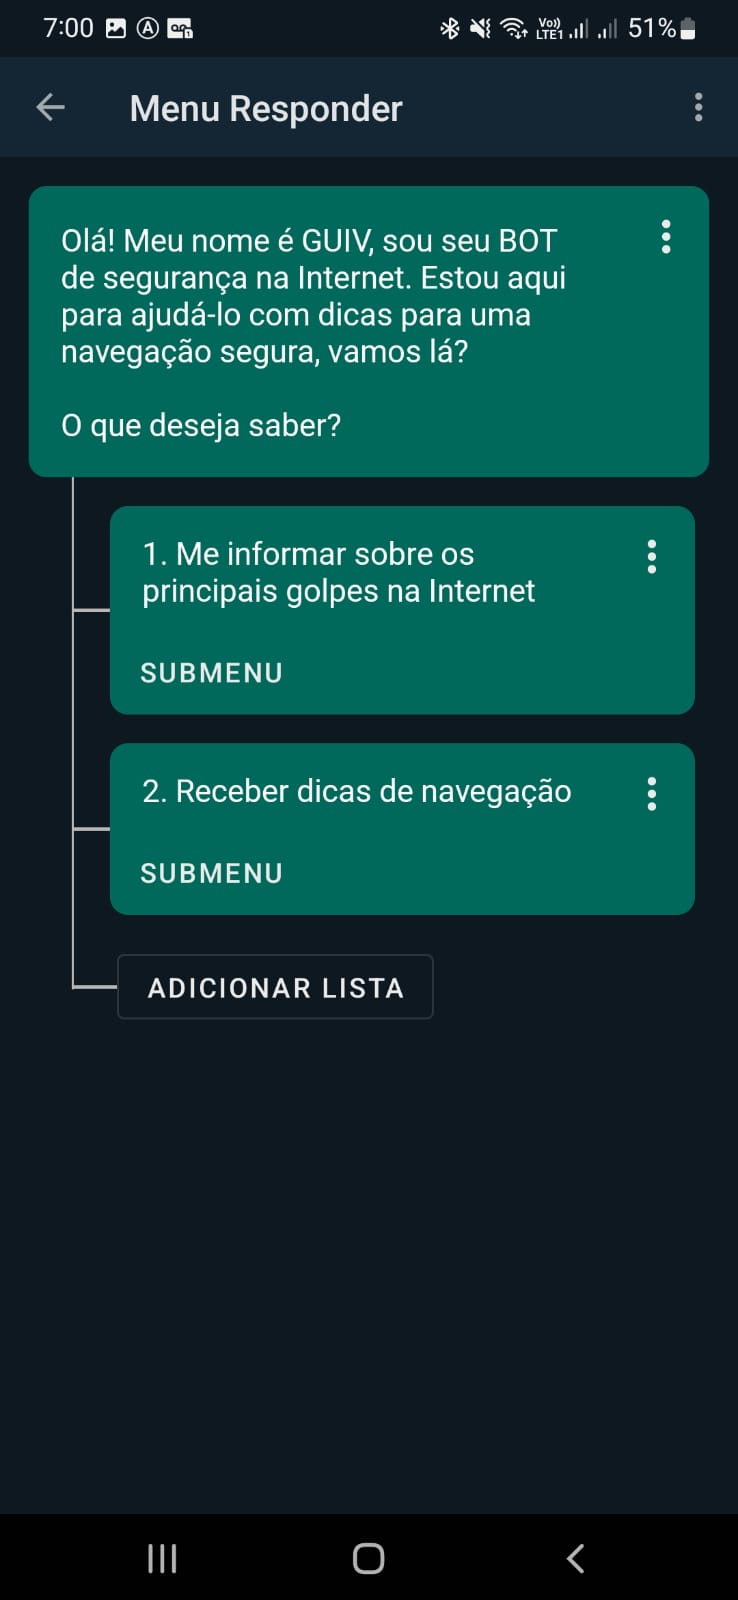
\includegraphics[width=6cm,height=8cm]{Partes/Imagens/Menu 3.jpeg}
\caption{Fonte: Whatsauto (2022).}
\end{subfigure}%
\end{figure}

        Mesmo depois de criado, se consegue editar e excluir as opções, basta clicar nos 3 pontinhos que ficam na direita de cada campo. \\

        Para que se crie as opções dentro de cada submenu, basta clicar em "SUBMENU" que fica em cada lista e ele te direcionará para a tela de criação dos submenus, que é igual a tela de criação do menu:

\begin{figure}[!htb]
\centering
\captionsetup[subfigure]{labelformat=empty}
\caption{``Submenu 1''}
\begin{subfigure}{.5\textwidth}
\centering
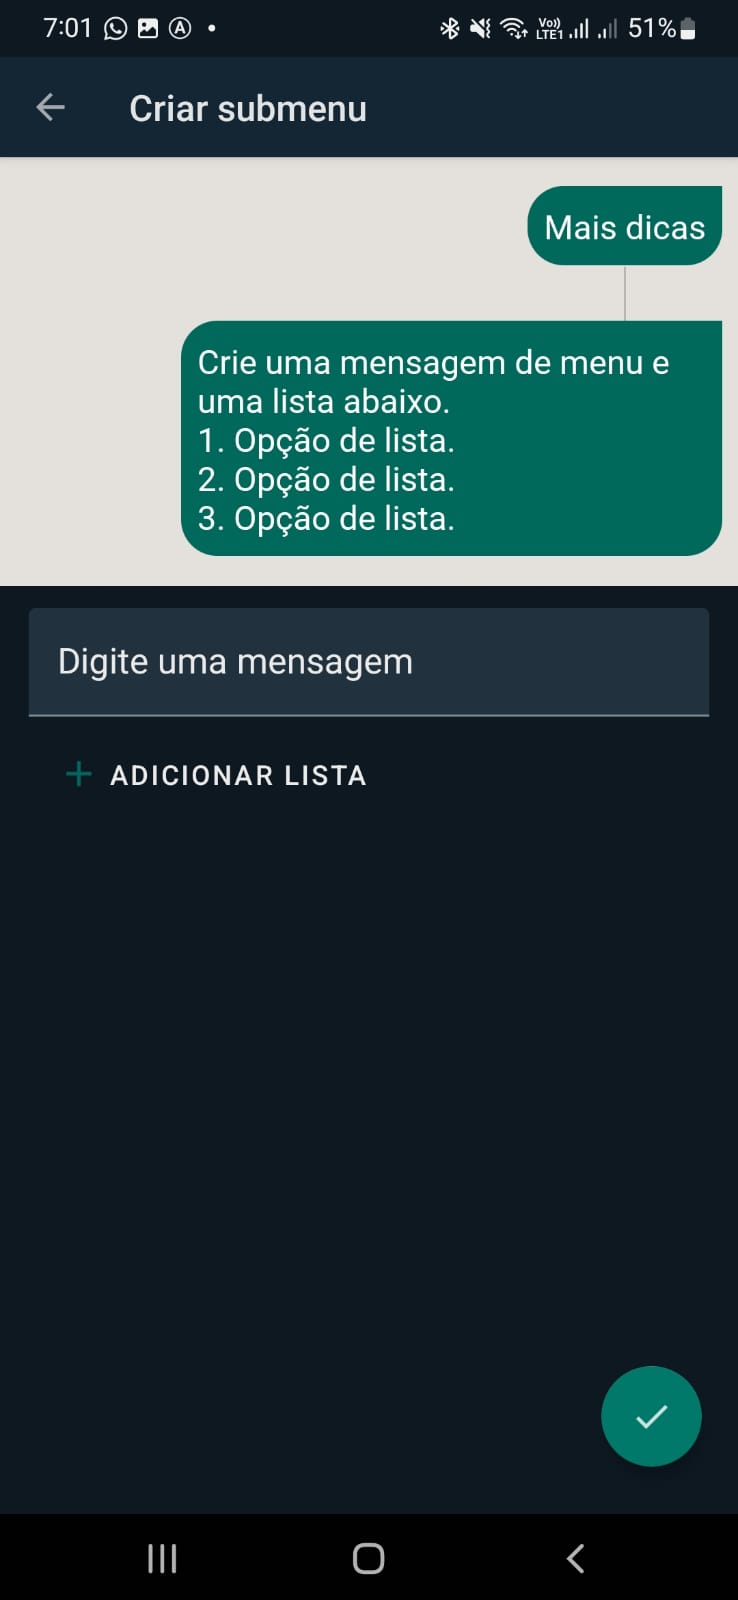
\includegraphics[width=6cm,height=8cm]{Partes/Imagens/Submenu 1.jpeg}
\caption{Fonte: Whatsauto (2022).}
\end{subfigure}%
\end{figure}


\begin{figure}[!htb]
\centering
\captionsetup[subfigure]{labelformat=empty}
\caption{``Submenu 2''}
\begin{subfigure}{.5\textwidth}
\centering
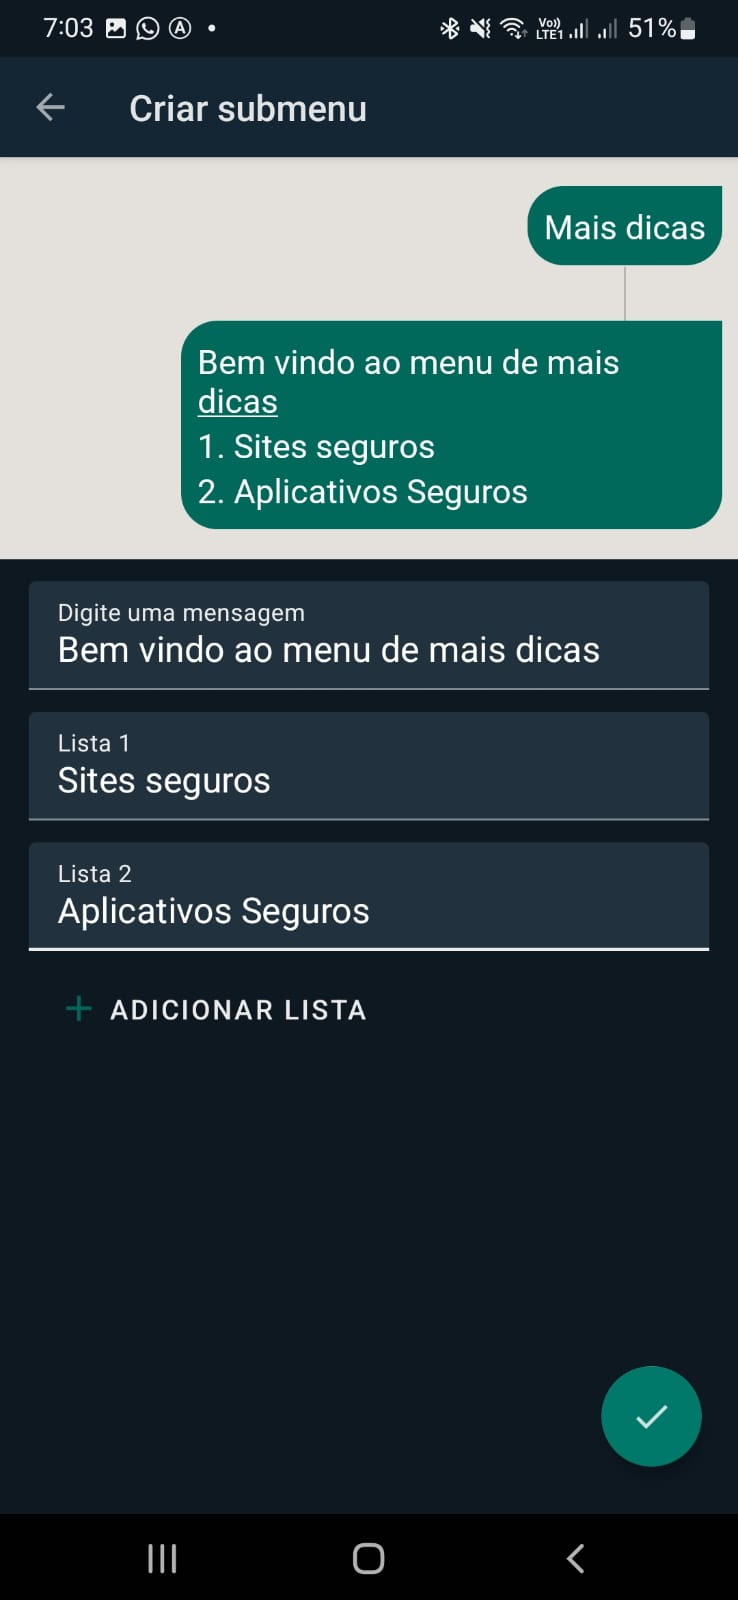
\includegraphics[width=6cm,height=8cm]{Partes/Imagens/Submenu 2.jpeg}
\caption{Fonte: Whatsauto (2022).}
\end{subfigure}%
\end{figure}

\begin{figure}[!htb]
\centering
\captionsetup[subfigure]{labelformat=empty}
\caption{``Submenu 3''}
\begin{subfigure}{.5\textwidth}
\centering
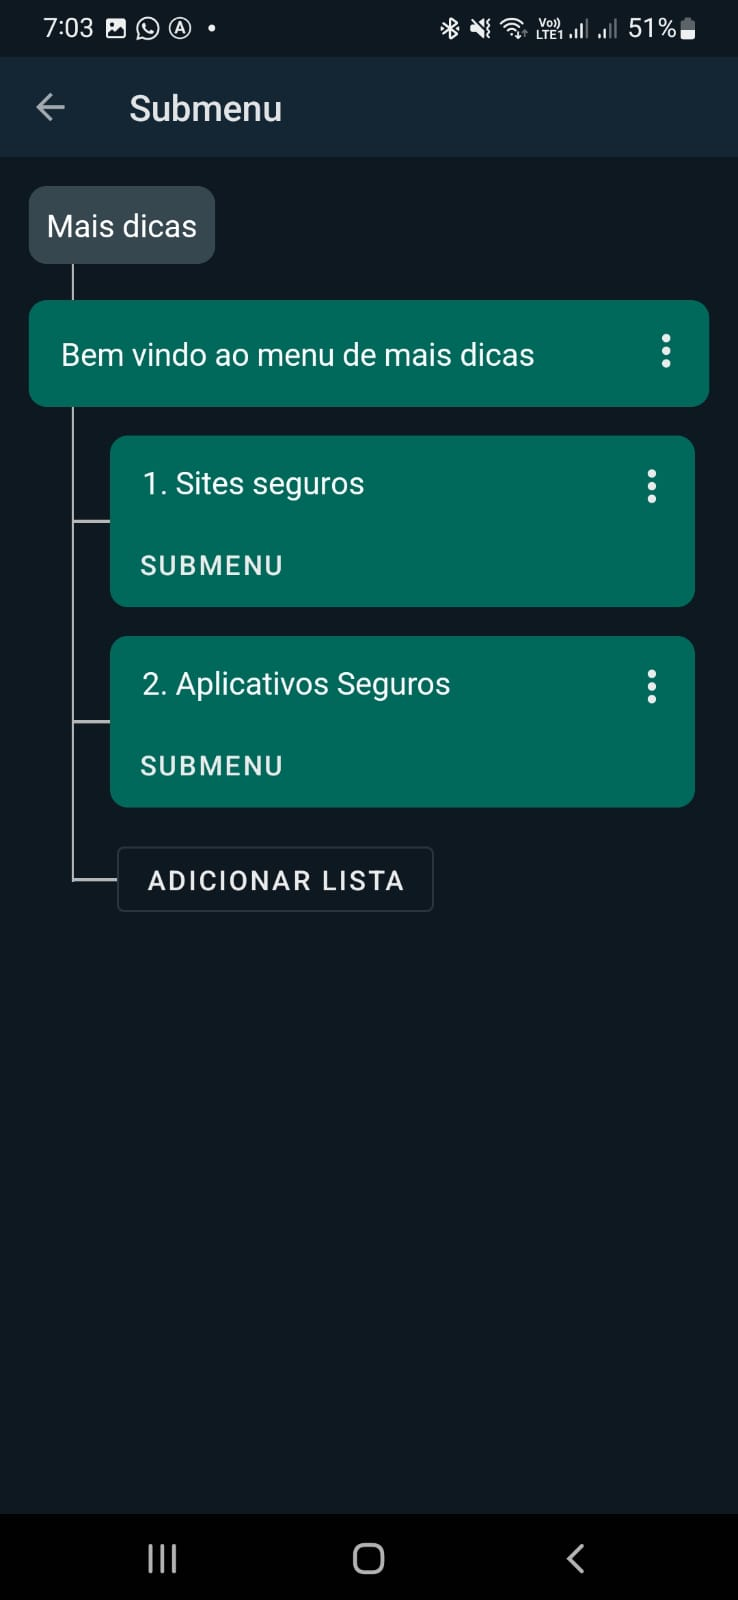
\includegraphics[width=6cm,height=8cm]{Partes/Imagens/Submenu 3.jpeg}
\caption{Fonte: Whatsauto (2022).}
\end{subfigure}%
\end{figure}

        \newpage
        
        Preenchendo os campos de texto e das listas seu submenu estará criado, podendo criar mais submenus dentro dele.
        
        Para colocar o BOT no ar, basta voltar para a tela de seleção do tipo de configuração e ir na categoria CASA na parte superior do aplicativo, dentro dela, você irá habilitar as respostas automáticas: \newpage

\begin{figure}[!htb]
\centering
\captionsetup[subfigure]{labelformat=empty}
\caption{``Menu Ligar 1''}
\begin{subfigure}{.5\textwidth}
\centering
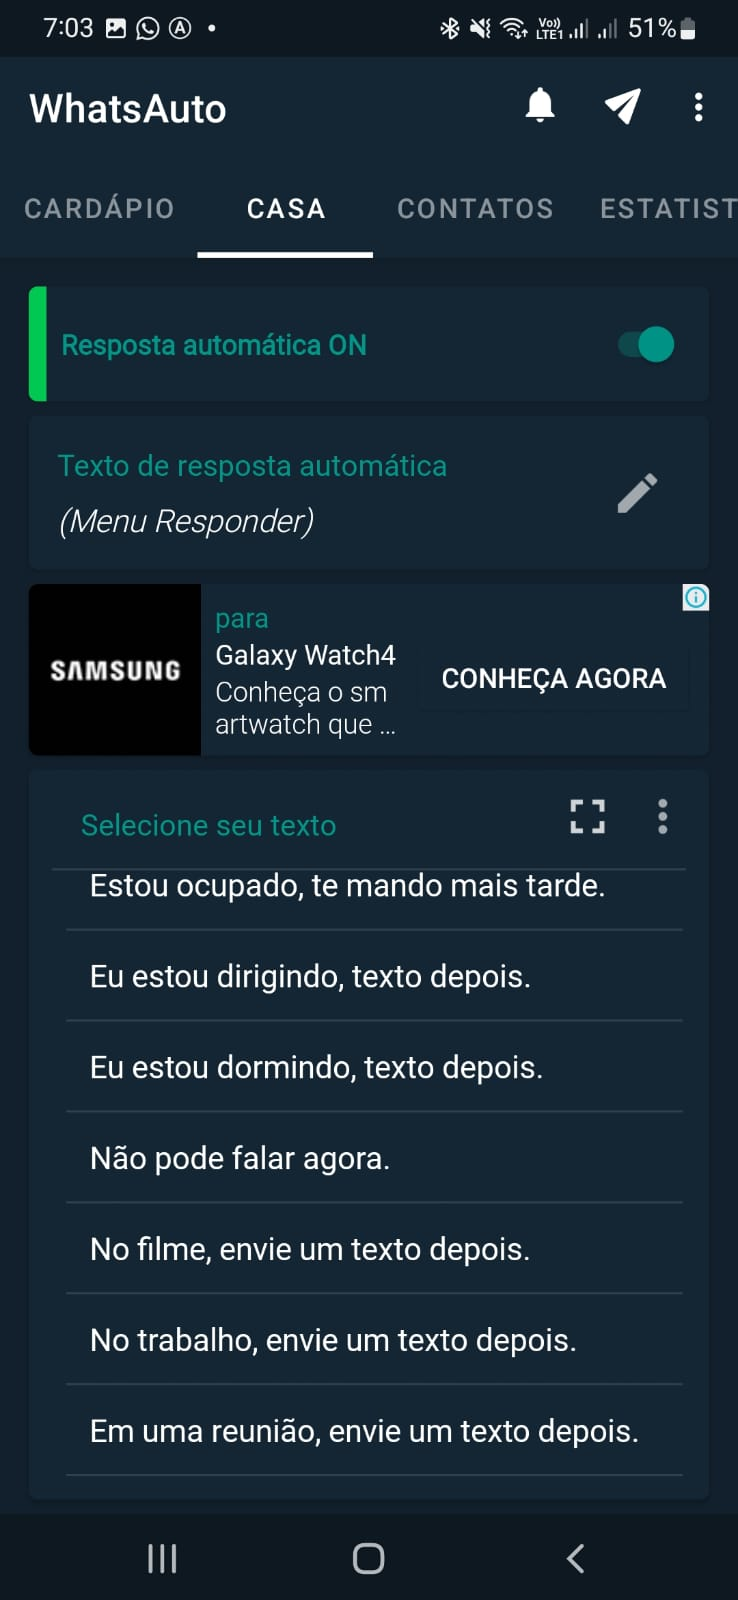
\includegraphics[width=6cm,height=8cm]{Partes/Imagens/Menu ligar 1.jpeg}
\caption{Fonte: Whatsauto (2022).}
\end{subfigure}%
\end{figure}

         E na parte do "texto de resposta automática", colocaremos a opção "Menu Responder", como mostra na imagem abaixo:

\begin{figure}[!htb]
\centering
\captionsetup[subfigure]{labelformat=empty}
\caption{``Menu Ligar 2''}
\begin{subfigure}{.5\textwidth}
\centering
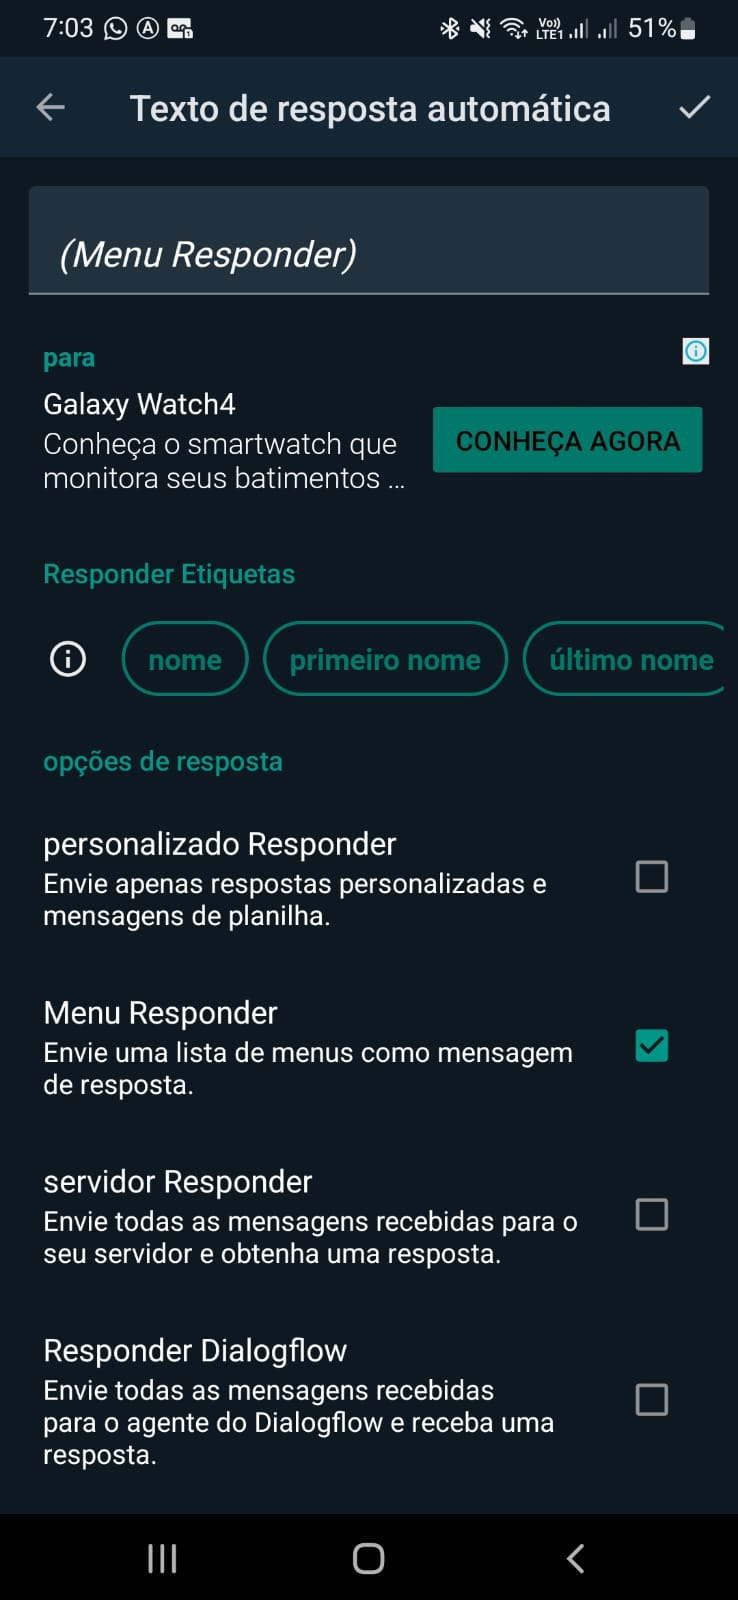
\includegraphics[width=6cm,height=8cm]{Partes/Imagens/Menu Ligar 2.jpeg}
\caption{Fonte: Whatsauto (2022).}
\end{subfigure}%
\end{figure}
\newpage
  
\section{Testes do Bot}
\subsection{Plano de testes:}

    Basicamente nós coletamos os feedbacks sobre a qualidade das informações passadas pelo BOT, entendimento de modo geral e usabilidade do layout do chat de WhatsApp.\\
	Diferente de outros BOTs, o nosso não possui a ferramenta de coleta de informações pessoais do usuário por meio de chat, nem uma IA \cite{ia}, para identificação linguística para maior aproximação com um atendente real, o que iria deixar mais natural e dinâmico as conversas com os usuários.\\
	Nós enviamos o link para algumas pessoas não envolvidas diretamente com nosso trabalho para testarmos todos os passos descritos acima. Obtivemos um resultado satisfatório e bem informativo, algumas criticas foram descritas, estamos fazendo de tudo para a correção futura.
\item \textbf{CRÍTICAS}: \\
Não tinha mensagem final ao parar de conversar com o BOT. \\
Falta do link na página do Instagram.\\
\item \textbf{ELOGIOS}: \\
“Um bom BOT bem útil, fácil de usar, tem só um atraso na resposta, mas nada que seja ruim ou que atrapalhe”\\
“No geral, está funcionando muito bem. Está bem resumido, porém explicativo”

\subsection{Resultado do plano de Testes:}

Foram feitos 8 testes com pessoas não relacionadas com nosso trabalho, 2 delas relataram problemas com o link do Instagram, o que nós não sabemos o porquê ocorreu. Várias ideias foram sugeridas pelos responsáveis pelos testes e algumas das ideias foram implementadas, por exemplo:\\
- Menu para sair da conversa\\
- Mensagem final agradecendo o teste e indicando nossa Pagina no Instagram. \\

\begin{figure}[!htb]
\centering
\captionsetup[subfigure]{labelformat=empty}
\caption{``Gráfico Pizza''}
\begin{subfigure}{.5\textwidth}
\centering
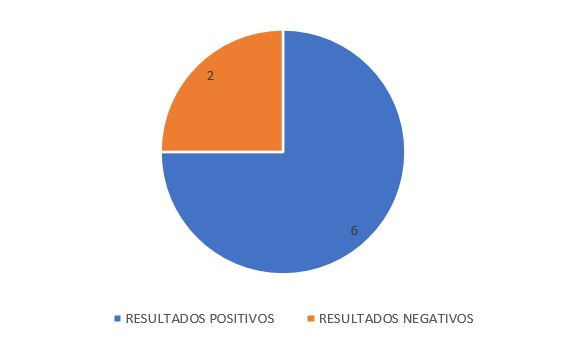
\includegraphics[width=8cm,height=6cm]{Partes/Imagens/Pizza.jpeg}
\caption{Fonte: Criado pelo autor (2022).}
\end{subfigure}%
\end{figure}

\newpage

\subsection{Imagens dos Testes:}

\begin{figure}[!htb]
\centering
\captionsetup[subfigure]{labelformat=empty}
\caption{``Teste 1''}
\begin{subfigure}{.5\textwidth}
\centering
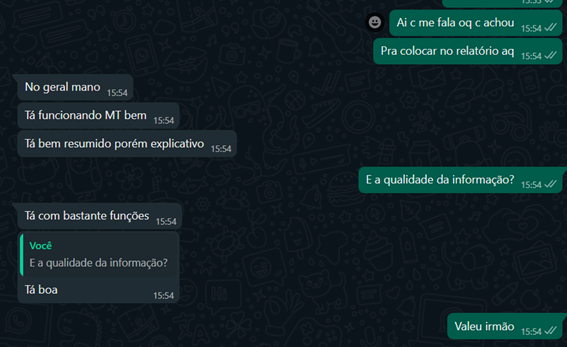
\includegraphics[width=6cm,height=8cm]{Partes/Imagens/teste 1.png}
\caption{Fonte: Criada pelo autor (2022).}
\end{subfigure}%
\end{figure}

\begin{figure}[!htb]
\centering
\captionsetup[subfigure]{labelformat=empty}
\caption{``Teste 2''}
\begin{subfigure}{.5\textwidth}
\centering
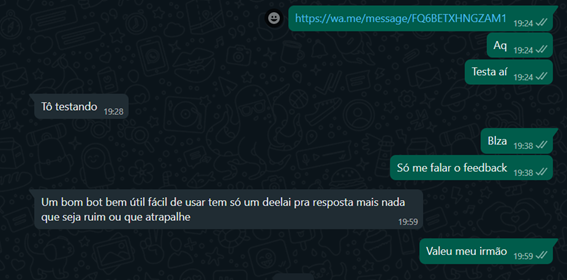
\includegraphics[width=6cm,height=8cm]{Partes/Imagens/teste 2.png}
\caption{Fonte: Criada pelo autor (2022).}
\end{subfigure}%
\end{figure}

\begin{figure}[!htb]
\centering
\captionsetup[subfigure]{labelformat=empty}
\caption{``Teste 3''}
\begin{subfigure}{.5\textwidth}
\centering
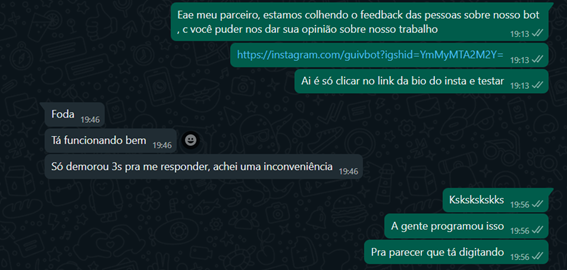
\includegraphics[width=6cm,height=8cm]{Partes/Imagens/teste 3.png}
\caption{Fonte: Criada pelo autor (2022).}
\end{subfigure}%
\end{figure}

\newpage

\subsection{Conclusões dos Testes:}

No geral foram obtidos bons resultados em todos os aspectos, as críticas foram recebidas muito bem. O resultado foi satisfatório. 

\section{Disponibilização do BOT}

 A plataforma que foi escolhida no projeto tem uma ampla vasta de disponibilização, porém a escolhida foi o WhatsApp, pois é um local onde os usuários tem mais acesso e disponibilidade para usar.
		
\end{itemize}

 
\chapter{\uppercase{Considerações finais}}
\label{conclusao}

A metodologia utilizada em sala para o desenvolvimento das atividades relacionadas ao trabalho de Projeto Integrador foi o SCRUM. \cite{scrum}\\

Em um mundo onde as pessoas estão cada vez mais envolvidas com a tecnologia, é de suma importância que os usuários estejam cientes de que para uma boa navegação é necessário ter conhecimento sobre os riscos que a internet oferece, como os dados ficam armazenados na web e quais são os cuidados que cada um deve ter ao acessar esses meios.  \cite{cookies}

Este projeto foi desenvolvido pensando em levar a informação para todos os tipos de usuário, sejam eles mais experientes ou menos. A criação do Bot Security teve como objetivo dois princípios: abordar sobre os principais tipos de golpes que estão sendo aplicados atualmente por meio da internet e oferecer algumas dicas para que o usuário tenha uma experiência mais segura na Web.\cite{segint} 

A entrega final do trabalho foi disponibilizada em uma rede social, o Instagram. Foi criada uma conta para divulgar o Bot e também abordar alguns temas estudados no 2º Período do Projeto Integrador para complementar o perfil e consequentemente levar mais conhecimento aos seguidores.

Apesar do objetivo final ter sido alcançado, houve alguns impasses durante a execução do projeto que fez com que o resultado final não saísse completamente da forma como planejado. O Bot teve que ser recriado e configurado 3 vezes devido as primeiras plataformas usadas para sua criação não serem gratuitas, o que gerou alguns atrasos e muito retrabalho. Em consequência deste atraso, alguns detalhes finais tais como configurações no Bot e plano de testes não puderam receber tanta atenção. Diante destes cenários, é concluído que para próximos trabalhos é preciso mais cautela e pesquisa antes de escolher plataformas que serão usadas no projeto. 

Em consideração as observações e pesquisas realizadas, foi possível detectar que a “Segurança na Internet” engloba aspectos bem mais amplos, pois envolve uma variedade de informações, dados pessoais e proteção à propriedade, e que se faz necessário aplicar conhecimento que visem ampliar a visão do usuário para que o mesmo busque mais entendimento, tornando-se consciente de suas ações na Web e contribuindo para um ambiente on-line pacífico.


 \section{Trabalhos Futuros}
  
Futuramente este trabalho pode ser complementado através de um aprimoramento nas configurações do BOT, como implementação de Inteligência Artificial, pois, atualmente o BOT está limitado a um menu de opções onde o usuário tem apenas a possibilidade de escolher uma das opções apresentadas. E com a Inteligência Artificial o usuário poderá ter uma experiência melhor e semelhante a de estar conversando com um atendente. 














\postextual %Indica início dos elementos pós-textuais	

    \bibliography{Referencias}

\begin{anexosenv}
% Imprime uma página indicando o início dos anexos
	%\partanexos

%(opcional)
\input{Partes/Anexo.tex} 
\end{anexosenv}

\end{document}
